\newcommand{\DpfGen}{\ensuremath{{\sf DPF.Gen}}}
\newcommand{\DpfEval}{\ensuremath{{\sf DPF.Eval}}}
\newcommand{\Dpf}{\ensuremath{{\sf DPF}}}
\newcommand{\DPF}{\ensuremath{{\sf DPF}}}
\newcommand{\Prg}{\ensuremath{{\sf PRG}}}
\newcommand{\Pbc}{\ensuremath{{\sf PBC}}}

\newcommand{\GenSched}{\ensuremath{{\sf GenSchedule}}}
\newcommand{\ServerPre}{\ensuremath{{\sf ServerPreprocess}}}
\newcommand{\ClientQ}{\ensuremath{{\sf ClientQuery}}}
\newcommand{\ServerA}{\ensuremath{{\sf ServerAnswer}}}
\newcommand{\ClientD}{\ensuremath{{\sf ClientDecode}}}
\newcommand{\get}{\ensuremath{\leftarrow}}
\newcommand{\Client}{\textsf{Client}~}
\newcommand{\Server}{\textsf{Server}~}
\newcommand{\CV}{\ensuremath{{\sf CV}}}

\renewcommand{\root}{\ensuremath{{\sf root}}}

\section{Distributed Point Function and 2-server PIR with Logarithmic Communication} %~\cite{boyle2016function}}

In earlier lectures, we learned an information-theoretic 2-server PIR
scheme 
by Dvir and Gopi~\cite{dvir20162}, which
achieves $n^{O(\sqrt{\log \log n / \log n})}$ communication per query. 
%We saw that in the IT-setting, the best known upper bound on the communication of 2-server PIR scheme is by Dvir and Gopi~\cite{dvir20162}.
%The scheme achieves $n^{O(\sqrt{\log \log n / \log n})}$ communication.
In this lecture, 
we will show how to get a 2-server PIR with logarithmic communication
%from only one-way functions (OWF).
relying only on a pseudorandom 
generator (PRG). This scheme is also interesting from a practical perspective
since in practice, we can use AES to realize
the PRG, and modern CPUs have hardware acceleration
for evaluating AES. 

Recall that 
from our undergraduate cryptography course, 
we know that the existence of a PRG
is equivalent to the existence of a one-way function (OWF)~\cite{haastad1999pseudorandom}.
Also, from an earlier lecture, we learned that any 1-server
classical PIR scheme 
with non-trivial bandwidth implies
Oblivious Transfer which cannot be constructed
in a blackbox manner from OWF~\cite{IR89}. 
Therefore, the scheme we will talk about today is in the 2-server setting.

%that if we are willing to assume that one-way functions (OWF) exist, we can construct a 2-server PIR scheme with $O(\log n)$ communication.
%\mingxun{I am not sure what other sschemes you want to compare to. The IT one seems to be the most appropriate one}

\subsection{Preliminary: Pseudorandom Generator}
%This scheme use pseudorandom generators (PRG). In particular, PRG implies the existence of OWF and OWF implies the existence of PRG~\cite{haastad1999pseudorandom}. 
We will rely on a pseudorandom generator (PRG),
which takes in a short random seed and expands
the seed to a longer pseudorandom string.

\begin{definition}[PRG]
    Let $\ell(\cdot)$ be a polynomial and let 
$G:  \{0,1\}^n \rightarrow \{0,1\}^{\ell(n)}$ be a deterministic
    polynomial-time algorithm. $G$ is a \Prg \ if it has the following properties:
    \hfill
    \begin{itemize}
        \item \textbf{Expansion:} $\forall n, \ell(n) > n$.
        \item \textbf{Pseudorandomness:} for any probabilistic polynomial-time distinguisher
$D$, there exists a negligible function ${\sf negl}(\cdot)$, 
such that 
        $$\left|\Pr_{r \getr \{0, 1\}^{\ell(n)}}\left[D(r) = 1\right] - 
\Pr_{s \getr \{0, 1\}^{n}}\left[D(G(s)) = 1\right]\right| \leq {\sf negl}(n)$$ 
        %Where $r \overset{{\scriptscriptstyle\$}}{\leftarrow} \{0,1\}^{l(n)}$ and
        %$s \overset{{\scriptscriptstyle\$}}{\leftarrow} \{0,1\}^{n}$.
    \end{itemize}
\end{definition}

\subsection{Distributed Point Function}

\begin{definition}[Point function]
A point function parametrized by some point $x \in \{0, 1\}^\ell$ 
is a function that evaluates to $1$ at $x$, and evaluates to $0$ 
everywhere else.
We will henceforth use the notation $P_x \{0,1\}^{\ell} \rightarrow \{0,1\}$
to denote a point function. 
By definition, $P_x(x) = 1$ and $P_x(x') = 0$ for $x' \neq x$.
%    For $x \in\{0,1\}^*$, the point function $P_{x}:\{0,1\}^{|{x}|} \rightarrow \{0,1\}$
%    is defined by $P_{x^*}(x^*) = 1 \ and \ P_{x^*}(x) = 0$ for all $x \neq x^*$.
\end{definition}

Boyle, Gilboa and Ishai~\cite{boyle2016function} introduced the concept of a distributed point function. 
A distributed point function
is a functional secret-sharing of a point function.
In this lecture, 
we will specifically focus on a {\it 2-way} secret sharing of a point function.
Essentially, given some point function $P_{x^*}$, 
one can ``secretly share'' the function to two keys $k_L,k_R$. 
Then, for party $t \in \{L, R\}$ which
receives the key $k_t$, 
%Then, if party $t\in\{0,1\}$ receives $k_t$, 
it can evaluate the function on any point $x$ and 
get a share of the outcome denoted $\Eval(k_t, x)$. 
It is guaranteed that in every point $x$, 
$\Eval(k_L, x)\xor\Eval(k_R, x)=P_{x^*}(x)$.
In other words, it is possible to combine
the two outcome-shares to reconstruct the  
evaluation of the point function at any point. 
Finally, security of the DPF requires that  
each party $t \in \{L, R\}$ does not learn  
the ``special point'' (i.e., $x^*$) given its individual key $k_t$.


\begin{definition}[2-share \Dpf]
    A DPF is a pair of possibly randomized 
algorithms (\Gen,\Eval) with the following syntax:
    \hfill
    \begin{itemize}
        \item $\Gen(1^\lambda,x^*)$: Outputs a pair of keys $k_L,k_R$.
        \item $\Eval(1^\lambda, k,x)$: Outputs the evaluation outcome $y \in \{0,1\}$.
    \end{itemize}
    \paragraph{Correctness.} 
Correctness requires that for any $\lambda$, 
any $\ell$, 
any $x^*, x \in \{0, 1\}^{\ell}$, 
\[
\Pr\left[k_L,k_R \leftarrow \Gen(1^\lambda, x^*):\Eval(k_L,x) \oplus \Eval(k_R,x) = P_{x^*}(x)\right] = 1
\]


\paragraph{Security.} 
Security requires that 
there exists a probabilistic polynomial-time simulator $\Sim$, 
such that 
for any $\ell = \ell(\lambda)$ that is a polynomial function in $\lambda$, 
and any $x^*\in \{0,1\}^{\ell(\lambda)}$, 
the following experiments are computationally indistinguishable
for both $t  = L$ and $t = R$: 
    \begin{itemize}
        \item $\mathsf{Real}(1^\lambda, x^*)$: $k_L,k_R\get  \Gen(1^\lambda, x^*)$ and output $k_t$;
        \item $\mathsf{Ideal}(1^\lambda)$: Output $\Sim(1^\lambda, \ell)$.
    \end{itemize}
\end{definition}
Intuitively, security requires that the any individual 
key $k_L$ or $k_R$ 
can be simulated without knowledge
of the special point $x^*$.

\subsection{DPF $\Longrightarrow$ 2-Server PIR}

Given a DPF scheme henceforth denoted $(\DpfGen, \DpfEval)$, 
we can construct 
a 2-server PIR scheme as follows.
Henceforth we use $\DB \in \{0, 1\}^n$ 
to denote the database.

%Let $\DB \in \{0,1\}^{n}, i \in [n]$ and $\lambda$ be the security parameter.
%Suppose we have an efficient 2-share binary DPF scheme $\DpfGen$ and $\DpfEval$, such that the key length is $O_\lambda(\log n)$ (where $n$ is the size of the input domain), and the evaluation algorithm is efficient. 
%Then, we can have the following 2-server PIR scheme. %n the following, when the context is clear, we will omit $1^\lambda$ in the description.

\begin{enumerate}
    \item Given the query $i$, the client 
computes $(k_L,k_R) \leftarrow \DPF.\Gen(1^\lambda, i)$
    \item The client sends %$(k_L,k_R)$ to 
$k_L$ to the left server and sends $k_R$ to the right server. 
%\Server 0 and \Server 1 respectively.
    \item %For 
Each server $t \in \{L, R\}$ receives $k_t$, 
and replies 
%$t\in\{0,1\}$, \Server $t$ responds with 
$y_t := \bigoplus_{j\in [n]} \DPF.\Eval(k_t,j)\cdot \DB[j]$;
    \item the client receives
$y_L$ and $y_R$ from the two servers respectively, 
and  outputs $y_L \oplus y_R$.
\end{enumerate}

\paragraph{Correctness.} 
It is not hard to check that the answer output by the client
is correct by the DPF's correctness:  
\begin{align*} 
    y_0 \oplus y_1 & = \left(\bigoplus_{j}\DB[j]\cdot \DpfEval(k_0,j) \right) \oplus \left(\bigoplus_{j}\mathsf{DB}[j]\cdot \DPF.\Eval(k_1,j) \right) \\
    & = \left(\bigoplus_{j}\DB[j]\cdot (\DpfEval(k_0,j)\xor \DPF.\Eval(k_1,j)) \right) \\
    & = \left(\bigoplus_{j}\DB[j]\cdot P_{i}(j)\right) \\
    & = \DB[i].
\end{align*}

\paragraph{Security.}
Security of the PIR follows directly from the security of the DPF.



\subsection{DPF Construction}

\begin{figure*}[t]
    \centering

    \begin{subfigure}{0.48\textwidth}
     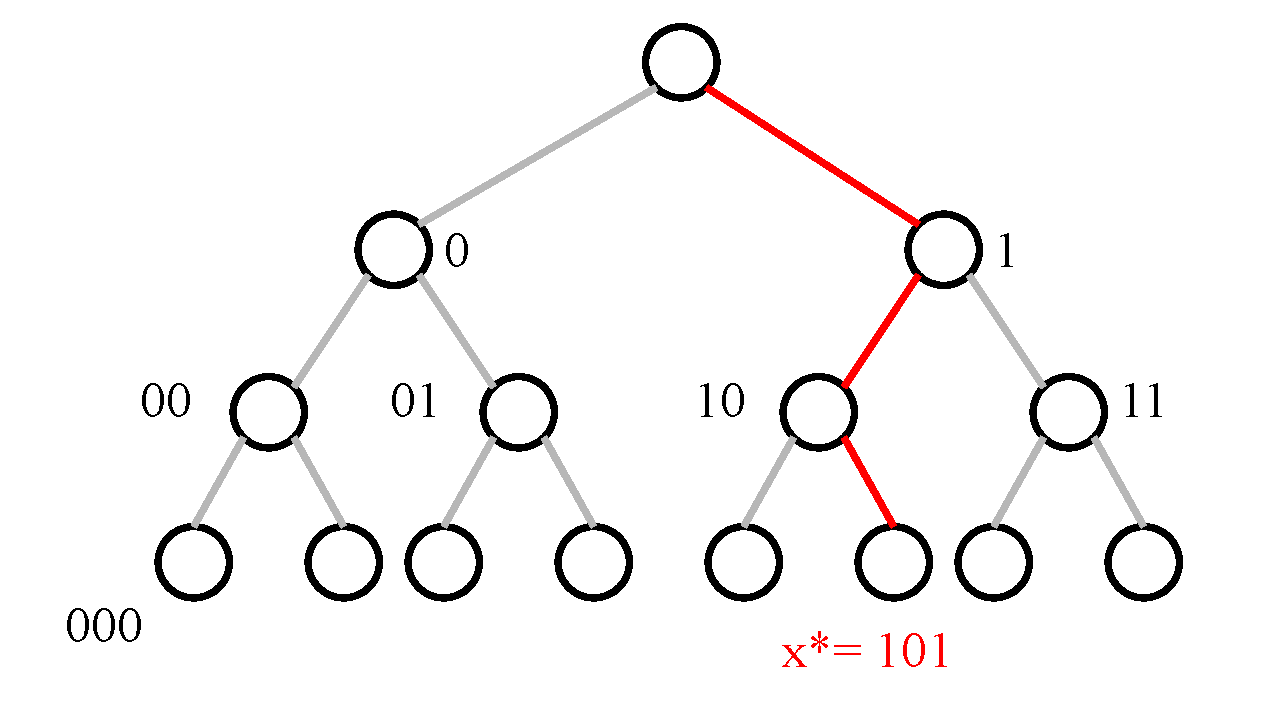
\includegraphics[width=\textwidth]{DPFtree.pdf}
     \caption{The binary tree structure used in DPF. Each node has a unique name. The path from the root to the leaf node $x^*$ is the ``special path''.}
\label{fig:tree}
    \end{subfigure}   
    \hfill
     \begin{subfigure}{0.48\textwidth}
        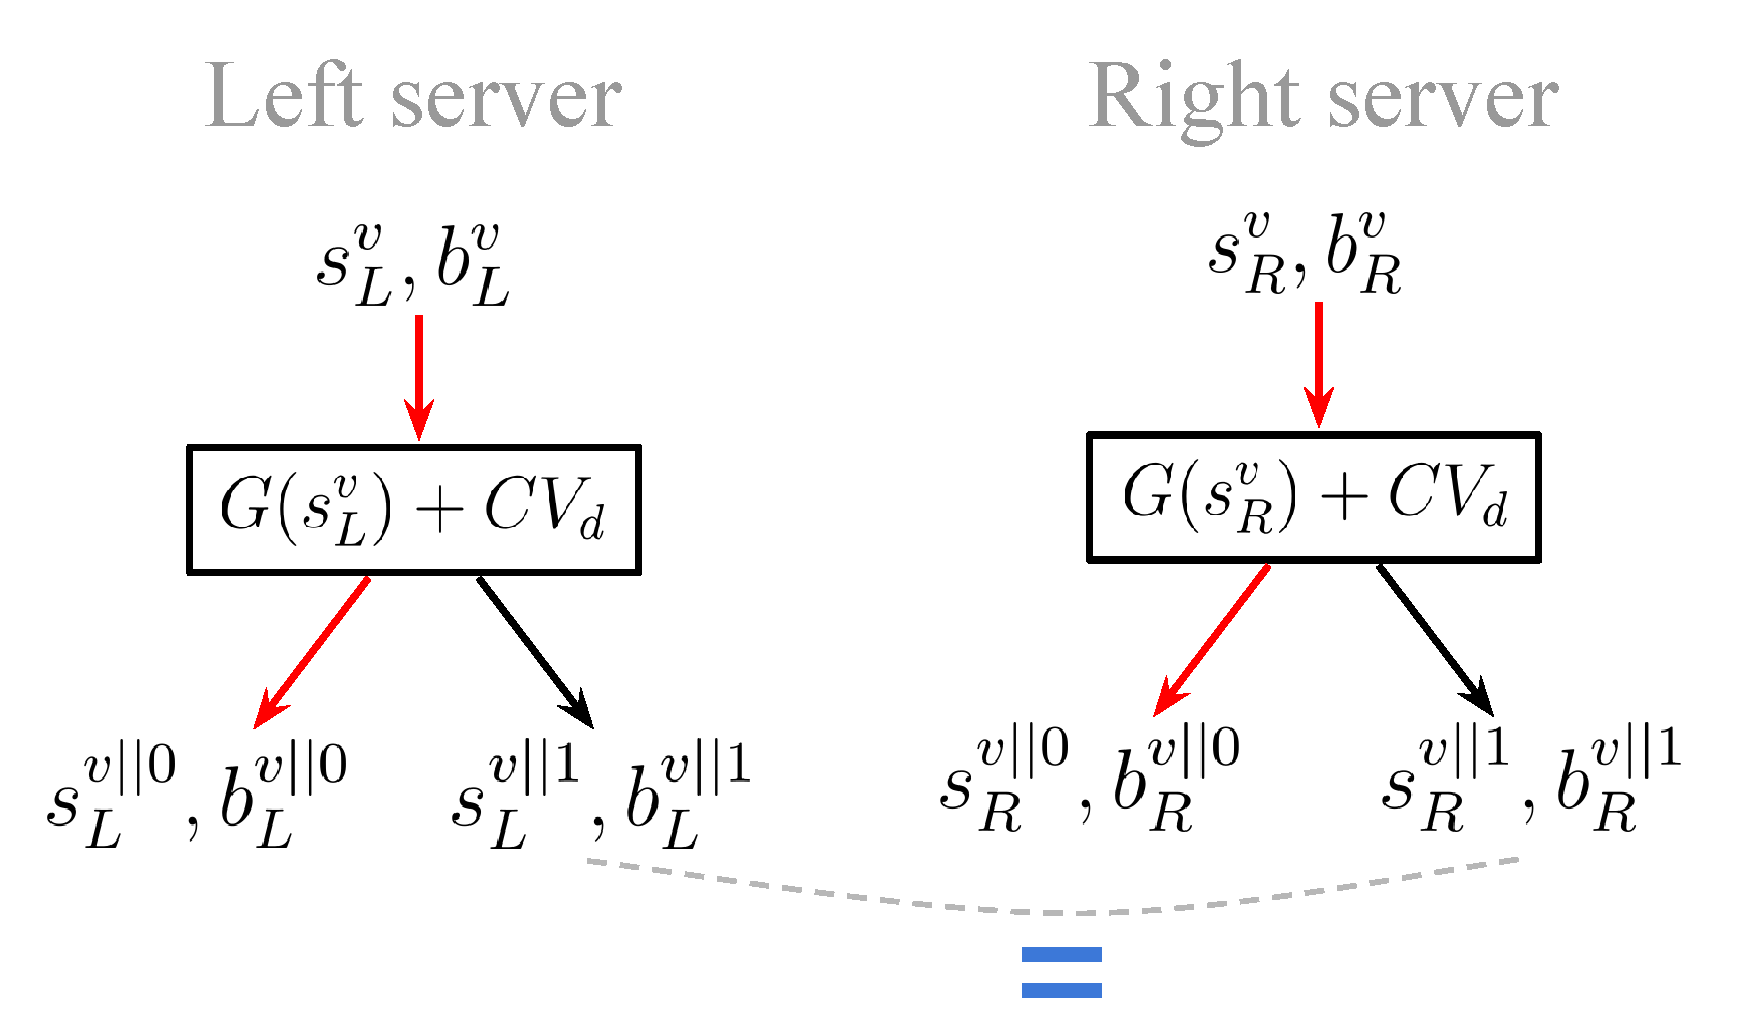
\includegraphics[width=\textwidth]{DPF1.pdf}
        \caption{Expansion during the evaluation algorithm.
The key generation computes the correction vector $\CV$ 
in a way that guarantees the following: 
for any $u$ not on the special
path, $(s_L^u, b_L^u) = (s_R^u, b_R^u)$;
and for any $u$ on the special path, 
$b_L^u \neq b_R^u$ and moreover,
the pair $(s_L^u, s_R^u)$ is indistinguishable
from two independent random strings.
%Expansion on the ``special path''. The construction enforces  the children not on the special path to have identical information, while maintaining the properties on the special path.
}
\label{fig:expand}
    \end{subfigure}
     \caption{Illustration of the DPF construction.\label{fig:dpf-demo}}
\end{figure*}





We now show how to construct an efficient DPF based on a pseudorandom
generator $G$:
 $$G: \{0,1\}^{\lambda} \rightarrow  \{0,1\}^{2\lambda + 2}. $$
The algorithm is based on a binary tree expansion idea.
%Where the series of evaluation results can be visualized as a binary tree.

\paragraph{Binary tree structure.}
Suppose we want to evaluate the DPF
at $n$ points denoted $0, 1, \ldots,  n-1$,
and we assume that $n$ is a power of $2$.

%To evaluate the DPF at all points $\{0, 1, \ldots, n-1\}$, 
Imagine that there is a binary tree
as depicted in \Cref{fig:tree}.
Each node in the tree has a name:  
the root's name is empty, and the two children of a node $v$ 
are named $v||0$ and $v||1$, respectively.
Henceforth, we say that the root is at {\it depth} $0$, the leaves
are at depth $\log n$, and so on.
Each leaf node corresponds to a point in 
$\{0, 1, \ldots, n-1\}$. In particular, it helps to express
each point in a binary representation.
For a point function $P_{x^*}$, 
the path from the root to the leaf node $x^*$ 
is called the special path highlighted in {\color{red}red}
in the figure. 

\paragraph{Key structure and evaluation algorithm.}
The DPF's $\Gen$ algorithm outputs two keys
$k_L = ((s_L, b_L), {\CV})$ and $k_R = ((s_R, b_R), {\CV})$,
where 
\begin{itemize}[leftmargin=7mm]
\item $s_L$ and $s_R$ are both $\lambda$-bit PRG seeds;
\item 
$b_L, b_R\in \{0, 1\}$ are flags indicating whether 
correction is necessary during the key expansion (see use
of the correction vector later in the algorithm). It
is guaranteed that $b_L \neq b_R$; 
and 
\item 
$\CV = (\CV_1, \ldots, \CV_{\log n})$ 
is a correction vector.
\end{itemize}

We will focus on the left server's perspective
for describing the evaluation algorithm. 
The right server's algorithm is the same except
that its input is $k_R$ instead of $k_L$.
Imagine that initially, the root of the tree is associated
with the pair $(s_L, b_L)$ which comes from $k_L$. 
Starting from the root, we will perform a key expansion
to compute a pair $(s_L^v, b_L^v)$
for every node $v$ in the tree.
 Each coordinate of the correction  
vector $\CV_1, \ldots, \CV_{\log n}$ 
will be consumed at each different level of the tree during the key expansion
process. 

More specifically, suppose some node $v$ has the pair
$(s_L^v, b_L^v)$, we can compute
the corresponding values at its two children $v||0$ and $v||1$ as follows
where $d$ denotes the depth of $v$'s children:
\[ 
(s_L^{v||0}, b_L^{v||0}), (s_L^{v||1}, b_L^{v||1}) \leftarrow G(s_L^v) \oplus
 \begin{cases} 
    {\bf 0} & \text{ if } b_L^v = 0; \\
    \CV_d &  \text { if } b_L^v= 1. \\
 \end{cases}
\]
Notice that the correction component $\CV_d$ is only applied if $b_L^v =1$.

At the end of the expansion process, 
for each leaf node $x$, let $b_L^x$ and $b_R^x$ be
the two bits associated with the leaf $x$ 
output by the left and right servers, respectively. 
The outcome of the DPF at point $x$ is then $b_L^x \oplus b_R^x$. 

\begin{figure*}[p]
    \begin{minipage}{\textwidth}
        \begin{mdframed}
            \begin{center}
                \textbf{Generation Algorithm:} $\Gen(1^\lambda, x^*)$
            \end{center}
            
            \paragraph{Initialization:} 
            %Repeat the following process $m$ times (indexed by $j$):
            \begin{itemize}
                \item Sample $s_L$, $s_R$ as two $\lambda$-bit random strings. 
                \item Sample a random bit $b_L$. Let $b_R=b_L\xor 1$. 
                \item Let $\{x^*[1],\dots,x^*[\log n]\}$ be $x^*$'s binary representation.
            \end{itemize}
            
            
            \paragraph{Constructing correction vectors:}  
            \begin{itemize}[label={},leftmargin=*]
                %\renewcommand\labelitemi{}
                \item Initialize $v$ to be an empty string.
                \item For $d\in \{1,\dots, \log n\}$: 
                \item 
                \begin{itemize}
                    %\item If $x^*[i]=0$, set ${\sf Keep}=L$. Otherwise, set ${\sf Keep}=R$.
                    \item Sample a random string $r\getr \{0,1\}^{\lambda}$.
                    \item Solve for 
$\CV_d\in\{0,1\}^{2\lambda+2}$ such that the following constraints
are satisfied:
                    \begin{enumerate}
                        \item[(1)] Let $(s^{v||0}_L, b^{v||0}_L), (s^{v||1}_L, b^{v||1}_L) \get G(s^v_L) \xor (b^v_L \cdot \CV_d)$; \hfill \textit{//~Expansion on the LHS}
                        \item[(2)] Let $(s^{v||0}_R, b^{v||0}_R), (s^{v||1}_R, b^{v||1}_R) \get G(s^v_R) \xor (b^v_R \cdot \CV_d)$; \hfill \textit{//~Expansion on the RHS}

\vspace{2pt}
                        \item[(3a)] If $x^*[d]=0$: add the following constraint: 
                        \begin{align*}
                            (s^{v||0}_L, b^{v||0}_L, s^{v||1}_L, b^{v||1}_L) \xor (s^{v||0}_R, b^{v||0}_R, s^{v||1}_R, b^{v||1}_R) = (r, 1, 0^{\lambda}, 0).
                        \end{align*}
                        \item[(3b)] If $x^*[d]=1$: add the following constraint: 
                        \begin{align*}
                            (s^{v||0}_L, b^{v||0}_L, s^{v||1}_L, b^{v||1}_L) \xor (s^{v||0}_R, b^{v||0}_R, s^{v||1}_R, b^{v||1}_R) = (0^{\lambda}, 0, r, 1).
                        \end{align*}
                        %\hfill \textit{(Force the $x^*[i]$ direction to be different and the other direction to be identical.)}
                    \end{enumerate}
%                    \item Solve the equation based on the invariant to get $\CV_d$. The equation is always solvable.
                    \item Let $v\get v||x^*[d]$.
                \end{itemize}  
            \end{itemize}
            \paragraph{Output:} Output the following $k_L, k_R$:
%that include the strings and bits on the root and the shared correction vectors:
            \begin{align*}
                k_L=(s_L, b_L, \CV_1,\dots,\CV_{\log n}) \\
                k_R=(s_R, b_R, \CV_1,\dots,\CV_{\log n})
            \end{align*}
            
        \end{mdframed}
    \end{minipage}
    \caption{DPF key generation algorithm.\label{fig:DPF}}
    %\caption{Detailed description of \name.\label{fig:single-server}}
\label{fig:gen}
\end{figure*}

%\begin{remark}
%Notice that if we only want to learn $\Eval(k, i)$ for a particular $i$, the computation cost will be $O(\log n)$ calls to the PRG, because we can focus on the path from the root to the $i$-th leaf and ignore other nodes.
%And on the path we only do $\log n$ expansions.
%However, if we want to evaluate $\Eval(k, i)$ for all $i\in[n]$, the computation cost will be $O(n)$ because we can simply do the evaluation on the whole tree. 
%\end{remark}



\paragraph{Key generation algorithm.}
The key generation algorithm samples  
random $s_L \getr \{0, 1\}^\lambda$ and $s_R \getr \{0, 1\}^\lambda$ 
at the root nodes for the left and right servers, respectively.
It chooses a random bit $b_L \getr\{0, 1\}$ 
and sets $b_R = b_L \oplus 1$.
Then, it will choose the correction vector $\CV_1, \ldots, \CV_{\log n}$
in a way such that 
the following {\bf invariants} are guaranteed for each
tree node $v$:

\begin{itemize}[leftmargin=7mm]
\item 
For every tree node $v$
that is not on the special path leading to $x^*$, 
it must be that $(s_L^v, b_L^v) = (s_R^v, b_R^v)$.
\item 
For every tree node $v$
that is on the special path leading to $x^*$, 
it must be that $b_L^v \neq b_R^v$,
and moreover, the pair $(s_L^v, s_R^v)$ 
is indistinguishable from two independent $\lambda$-bit random 
strings.
\end{itemize}

Note that for some node $v$, if 
$(s_L^v, b_L^v) = (s_R^v, b_R^v)$
is already guaranteed, then 
for any node $u$ that is in the 
subtree of $v$,  
$(s_L^u, b_L^u) = (s_R^u, b_R^u)$
is automatically guaranteed because
the left and right servers
will behave identically when the apply the same 
expansion algorithm to compute 
all values in the subtree of $v$.
Therefore, in the key generation algorithm, 
we can compute the correction vector $\CV$
using only the special path, to maintain
the aforementioned invariants. 

The detailed key generation algorithm is specified
in \Cref{fig:gen}.
It is not hard to see that 
the key size is $\lambda+1+\log n\cdot (2\lambda+2)=O_\lambda(\log n)$.



%\paragraph{The key structure.} The $\Gen$ algorithm outputs two keys, $k_L, k_R$. For each key $k_t$ where $t\in\{0,1\}$, it contains the ``root'' information as a $\lambda$-bit random string $s$ and a bit $b\in\{0,1\}$. It also contains $\log n$ ``correction vectors'' $\CV_1, \dots, \CV_{\log n}$, each of size $2\lambda+2$ bit. $k_L, k_R$ will share the same sets of correction vectors. 
%We will see how they are constructed later. 



\ignore{
\paragraph{Evaluation algorithm.} 
Given a key containing $s,b$ and $\CV_1,\dots,\CV_{\log n}$, the evaluation algorithm is as follows.
We consider a binary tree with $\log n + 1$ levels and $n$ leaves (assume $n$ is a power of 2). 
The root is on the $0$-th level and the leaves are on the $\log n$-th level.
For the $2^i$ nodes on the $i$-th level, we use $i$-bit to label them: the labels are from $\underbrace{0,\dots,0}_{i~\text{bits}}$ to $\underbrace{1,\dots,1}_{i~\text{bits}}$.
The root is labeled with an empty string.
See Figure~\ref{fig:dpf-demo} for the demonstration.
Now given the string $s^v$ and the bit $b^v$ on a node $v\in \{0,1\}^{i-1}$ on the level $i-1$, the strings and the bits on the nodes $v||0$ and $v||1$ are:
\[ 
s^{v||0} || b^{v||0} || s^{v||1} || b^{v||1} \leftarrow G(s^v) \oplus
 \begin{cases} 
    0 & b^v = 0; \\
    \CV_d & b^v= 1. \\
 \end{cases}
\]
That is, $s^{v||0}, b^{v||0}$ are the string and bit on its left child, and $s^{v||1}, b^{v||1}$ are the string and bit on its right child.
We first use the PRG to expand $s^v$, then if $b^v=1$, we will apply the correction vector to the evaluation results. 
Finally, given the evaluation point $i\in[n]$, the bit on the $i$-th leaf will be $\Eval(k, i)$.

Notice that if we only want to learn $\Eval(k, i)$ for a particular $i$, the computation cost will be $O(\log n)$ calls to the PRG, because we can focus on the path from the root to the $i$-th leaf and ignore other nodes.
%And on the path we only do $\log n$ expansions.
However, if we want to evaluate $\Eval(k, i)$ for all $i\in[n]$, the computation cost will be $O(n)$ because we can simply do the evaluation on the whole tree. 
}




\ignore{
\paragraph{Generation Algorithm.} The generation algorithm needs to generate two correlated keys, such that when we look at the bit at the $x$-th leaves on the left server and the right server, (say $b^{x}_{L}$ and $b^{x}_{R}$), it must that $b^{x}_{L}\xor b^{x}_{R}=P_{x^*}(x)$. In fact, we want to ensure the following stronger properties.
Say on a particular node $v$, we denote the information evaluated by the left server and the right server as $(s^v_L,b^v_L)$ and $(s^v_R,b^v_R)$, respectively.
We also denote the path from the root to the $x^*$-th leaf as the ``special path''.

\begin{enumerate}
    \item If the node $v$ is on the special path (i.e., $v$ is a prefix of the binary representation of $x^*$), then $b^v_L\ne b^v_R$, and $s^v_L$ and $s^v_R$ are independent.
    
    \item Otherwise, $(s^v_L,b^v_L)=(s^v_R,b^v_R)$.
\end{enumerate}

The properties also hold for the leaf nodes, which is sufficient to prove the correctness of the DPF. 
We now see the how to ensure these properties.
We have the first lemma, which can be proved by a simple induction argument.
}

\ignore{
\begin{lemma}
    If on some particular node $v$, $(s^v_L,b^v_L)=(s^v_R,b^v_R)$, then the information on the subtrees of $v$ will be identical, regardless of $\CV_1,\dots,\CV_{\log n}$. That is, for every $v'$ that has prefix $v$, $(s^{v'}_L,b^{v'}_L)=(s^{v'}_R,b^{v'}_R)$. 
\end{lemma}

This lemma shows that we only need to focus on the ``special path''. We can sample the roots first by sampling two random strings $s_L,s_R$ and let $b_L$ and $b_R$ be two different bits. 
Then, we can just ``simulate'' the expansion process on the special path, and then set up the correction vector according to the target properties. 
Given a node $v$ on the special path ($v$ is a prefix of $x^*$), say $v$ is on the $i-1$ level.
Now assuming the correction vector $\CV_i$ is a \textit{variable} to be determined.
We can still following the evaluation algorithm, but all the expansion results, $s^{v||0}_L, b^{v||0}_L, s^{v||1}_L, b^{v||1}_L$, $s^{v||0}_R, b^{v||0}_R, s^{v||1}_R, b^{v||1}_R$, will be temporally some linear expressions of the variable $\CV_i$.
Then, we can enforce the invariants.
Say $v||0$ is still the prefix of $x$ (the other case is symmetric). We require that 
\begin{itemize}
    \item \textit{Invariant on the special path.} 1) The xor-sum of $s^{v||0}_L$ and $s^{v||0}_R$ is a freshly sample random string $r$ (ensuring they are independent); 2) $b^{v||0}_L$ and $b^{v||0}_L$ are different.
    \item \textit{Invariant on other nodes.} $(s^{v||1}_L,b^{v||1}_L)=(s^{v||1}_R,b^{v||1}_R)$.
\end{itemize}
Now these invariants set up a simple linear equation and we can easily solve the value of $\CV_i$.
The equation is always solvable because $b^v_L$ and $b^v_R$ are different.
Thus, the $\CV_i$ will always and only affect the expansion on the one side.
Note that the second invariant just enforces that the whole subtree of $v||1$ will be identical, and we just need to go to the child $v||0$ and derive $\CV_{i+1}$ based on $s^{v||0}_L, b^{v||0}_L$ and $s^{v||0}_R, b^{v||0}_R$.
We run this algorithm from level $1$ to level $\log n$ and get $\CV_1,\dots,\CV_{\log n}$.
The algorithm is presented in Figure~\ref{fig:DPF} and an example is presented in Figure~\ref{fig:dpf-demo}.
}

\paragraph{Analysis.}
The correctness can be verified by 
inductively checking that the aforementioned invariants hold
at every level.  

%doing an induction proof from level $1$ to level $\log n$.

Security can also be proven inductively.
We prove left-server security below since right-server security is symmetric.
Henceforth, we use $x^*[:d]$ to denote the first $d$ bits of the
binary representation of $x^*$.
For the base case, observe that the terms $(s_L, b_L)$  are random
and independent of $s_R$. 
Now, suppose that 
the joint distribution of $(s_L, b_L, \CV_1, \ldots, \CV_{d-1})$
and  $s_R^{x^*[:d-1]}$ are indistinguishable from random. 
We want to inductively prove that 
the joint distribution of $(s_L, b_L, \CV_1, \ldots, \CV_d)$
and  $s_R^{x^*[:d]}$ are indistinguishable from random.
Without loss of generality, assume that $x^*[d] = 0$
since the other direction is symmetric.
Let $v = x^*[:d-1]$, observe
that 
\[\CV_d = 
(s_L^{v||0}, b_L^{v||0}, s_L^{v||1}, b_L^{v||1}) \xor 
(s_R^{v||0}, b_R^{v||0}, s_R^{v||1}, b_R^{v||1}) \xor 
%\begin{cases}
(r, 1, 0, 0) %& \text{ if } x^*[d] = 0 \\
%(0, 0, r, 1) & \text{ if } x^*[d] = 1
%\end{cases}
\]
By our induction hypothesis, given $(s_L, b_L, \CV_1, \ldots, \CV_{d-1})$,
$s_R^v$ is indistinguishable from random.
Due to the security of the PRG, 
$(s_R^{v||0}, b_R^{v||0}, s_R^{v||1}, b_R^{v||1}) = G(s_R^v)$ 
is indistinguishable from random 
given $(s_L, b_L, \CV_1, \ldots, \CV_{d-1})$.
Therefore, given 
$(s_L, b_L, \CV_1, \ldots, \CV_{d-1})$,
$\CV_d$ 
is indistinguishable from random.
Further, note that $s_R^{v||0} = \CV_d[:\lambda] \xor r$
where $r \getr \{0, 1\}^\lambda$ is a fresh random string
of length $\lambda$.
This means that 
given $(s_L, b_L, \CV_1, \ldots, \CV_{d-1})$, 
both $\CV_d$ and $s_R^{v||0}$
are indistinguishable from fresh random strings.

%Given $(s_L, b_L)$ which is part of the left server's key,
%the terms $(s_R^{v||0}, b_R^{v||0}, s_R^{v||1}, b_R^{v||1})$
%are indistinguishable from random. 


%The security analysis is referred to~\cite{boyle2016function}. 
%\elaine{prove security?}


 \section{Batch PIR}

 \subsection{Motivation}
    So far, every PIR scheme we have seen only retrieves 1 bit at a time. 
    In many use cases, the client may want to fetch up to $Q$ database entries at the same time. 
    The navie solution is just to repeat the single-query algorithm $Q$ times.
If each instance
requires $O(n)$ computation for example,
then together all $Q$ instances 
would require $O(n \cdot Q)$ computation.
%    For instance, to compute $Q$ queries using a single-query PIR scheme with $O(n)$ computation, it requires $O(Qn)$ computation.
Batch PIR aims to handle a batch of queries at the same time, 
reducing the amortized cost.
We shall assume that $Q = o(n)$ since otherwise 
the server can just send the entire database to the client. 

     
\subsection{Batch PIR Based on Balls-and-Bins Hashing}

Given an $n$ bit long database and $Q=o(n)$ queries, we load-balance the database into $\frac{Q}{\log Q}$ buckets -- we use a hash function to hash each database entry to a bucket (by hashing their index).
Then, given the $Q$ queries, we again use the hash function to place the queries to the buckets. 
In expectation, each bucket will have $\log Q$ queries. 
Based on the balls-into-bins argument, each bucket will have no more than $\lambda \log Q$ queries with $1-\negl(\lambda)$ probability.
Therefore, we just do $\lambda \log Q$ PIR queries in each bucket (possibly dummy queries) to retrieve the target entries. 
This ensures the success probability is at least $1-\negl(\lambda)$.

\paragraph{Security.}
We are always making fix number of queries ($\lambda \log Q$ PIR queries in each bucket), so the scheme is secure by a reduction to the security of the underlying PIR scheme.

\paragraph{Cost.}
Moreover, say the underlying single-query PIR computation cost is linear in the size of the database.
We are making $\lambda \log Q$ queries to each bucket, and the total size of the buckets is just $n$. 
Therefore, the total computation cost is $O(\lambda \log Q n)$. 
So if $Q>\lambda \log Q$, this simple scheme saves computation.


     
     
\subsection{Cuckoo Hashing based scheme~\cite{angel2018pir}}

Angel et al.~\cite{angel2018pir} proposed SealPIR that uses cuckoo hashing to do batch PIR.
    
    \paragraph{Cuckoo Hashing}
    \begin{definition}[Cuckoo hashing]
        Given $n$ balls, $b$ buckets, and $w$
independent hash functions $h_0$, $\cdots$ , $h_{w}$ that map a ball to a
random bucket, compute $w$ candidate buckets for each ball by
applying the $w$ hash functions. For each ball $x$, place $x$ in any
empty candidate bucket. If none of the $w$ candidate buckets
are empty, select one at random, remove the ball currently in
that bucket ($x_{\text{old}}$), place $x$ in the bucket, and re-insert $x_{\text{old}}$. If
re-inserting $x_{\text{old}}$ causes another ball to be removed, this process
continues recursively until we finish the insertion or a maximum number of iterations is achieved.
    \end{definition} \
    
\paragraph{Batch PIR based on Cuckoo Hashing.}   
The scheme is as follows.
\begin{itemize}
    \item \textbf{Serer encoding.} Given an $n$ bit database, $b$ buckets, and $w$ hash functions, we hash each entry in the database (using their index as the key) to all $w$ candidate buckets and store it there.
    This results in a encoded database that each original entry is replicated $w$ times.
    The server will share the hash functions to the client.
    
    \item \textbf{Client scheduling.} Given the $Q$ queries, the client use the cuckoo hashing method to insert (or say, schedule) the queries to the buckets (again, using the indices as the keys).
    Our target is that each bucket has at most one query, and all query can be inserted in one of its candidate bucket.
    
    \item \textbf{Client query.}. Now the client just makes one query in each bucket. If the client successfully insert all queries earlier, it can then proceed to learn all the target entries because the server has inserted the entries in all the candidate buckets.
\end{itemize}

An example can be found in Figure~\ref{fig:sealpir}.
   
The authors used 3 hash functions for encoding and set the number of buckets $b = 1.5Q$. For $Q\geq 200$, the author showed that the chance of failure during
the scheduling phase is $\leq 2^{-40}$.
Notice that this is not cryptographically neligible. 
To enforce negligible failure probability, we can introduce a size $\lambda$ stash of the cuckoo hash table.
That is, the stash stores at most $\lambda$ elements that fail to be inserted. 
Then, the client also has to make additional $\lambda$ PIR queries to the whole database.
This ensures the failure probability to be $\negl(\lambda)$.

\paragraph{Cost Analysis.} 
Assume the underlying single-query PIR scheme is linear.
The client will make one query in each bucket and the total bucket size is $wn$.
Also, the client needs to make $\lambda$ additional query to the whole database to ensure negligible failure probability.
Then, the computation cost for the $Q$ queries are just $(w+\lambda)n$.

    
    
\begin{figure*}
    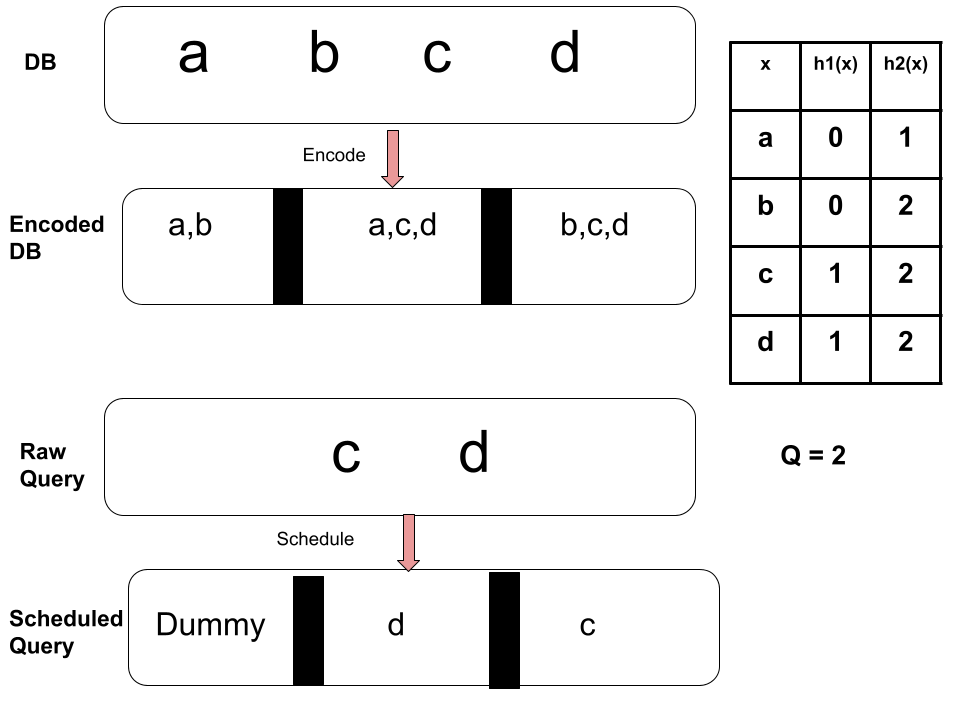
\includegraphics[scale=0.45]{scribimg_batchpir.png}
    \caption{An example of the cuckoo hashing based batch PIR. \label{fig:sealpir}}
\end{figure*}












\ignore{

%%%%%%%%%%%%%

Intuitively, this just applies all hash functions to an entry. If all buckets it gets hashed to are
taken, it will choose a random bucket, remove the ball currently in there and re-insert
using the same procedure. \\
\paragraph{Probabilistic Batch Codes}
\begin{definition}[Batch Code ~\cite{angel2018pir}]
    A (n, m, k, b)-batch code B takes as input a collection DB of n
    elements, and produces a set of m codewords, C, distributed
    among b buckets. Formally, $B : DB \rightarrow (C_0,..., C_{b})$, where
    $|Ci|$ is the number of codewords in bucket i, and the sum of
    codewords across all buckets is $m = \sum_{i=0}^{b-1}|Ci| \geq n$.
    The goal of these codes is two-fold. First, they ensure that any k elements
    from DB can be retrieved from the b buckets by fetching at most
    one codeword from each bucket. Second, they keep the number
    of total codewords, m, lower than $k \cdot n$.
\end{definition}
Batch codes incur a large network overhead by guaranteeing completeness in that it
is always possible to retrive k codewords by querying k distinct buckets. By adding possibility of failure p,
bandwidth can be shaved off at the cost of a chance of query failure. Applying this relaxation
results in a Probabilistic Batch Code, which is how SealPIR is able to encode a database
into multiple sub-databases that can be queried simultaneously with PIR. Informally, they are defined by 3 functions:
\begin{itemize}
    \item \textbf{\sf Encode(DB):} Split the database and replicate entries accordingly.
    \item \textbf{\sf GenSchedule(W):} Generate a query to each subdatabase such that all desired items are retrieved.
    \item \textbf{\sf Decode(I):} Extracts individual responses from the server response.
\end{itemize}
A formal definition and construction using reverse hashing can be found on page 6 of ~\cite{angel2018pir}


\subsection{The SealPIR scheme}

\paragraph{Intuition} The main idea is to build a \Pbc \ over the PIR database. The only major modifications
are to GenSchedule and Decode, where the equeries must be modified to be PIR queries. While failures in the query scheduling phase are
possible, the authors tune the parameters to make the likelihood very low.
\\
\paragraph{Notation}
Let \Pbc = $(\mathsf{Encode},\GenSched,\mathsf{Decode})$ be a Probabilistic Batch code constructed using Cuckoo hashing. Additionally,
Let PIR = (\ServerPre,\ClientQ,\ServerA,\ClientD) be a PIR scheme.

\paragraph{\sf SealPIRPreprocess} Given w independent hash functions $H = (h_1,...,h_w)$ and \DB, output b buckets $B = {B_1,...,B_b}$, where:
$$\sf B_i = SealPIRPreprocess(s_i),(s_0,...s_b) = encode(DB) $$
\paragraph{\sf SealPIRQuery} For a set of Q queries $q_1,...,q_b$, and Cuckoo hashing algorithm CK:
\begin{enumerate}
    \item Client computes $\sigma \leftarrow GenSchedule(Q)$
    \item if $\sigma \neq \perp$ goto (3) else  return failure
    \item Client computes $(q_1,...q_b) \leftarrow (ClientQuery(B_0,\sigma[0]),...,ClientQuery(B_Q,\sigma[b]))$ and sends the result to the server
\end{enumerate}
Where $\sigma \in \{\{1,....,b\}\}^b$ maps queries to the bucket the query should go to. $\sigma == \perp$ if there were two indices mapped to the same bucket.

\paragraph{\sf SealPIRAnswer} Server computes and sends $$r_i = \ServerA(B_i,\sigma[i]), \forall i \in [Q]$$ back to client.
\paragraph{\sf SealPIRDecode} To retreive the answer to the ith query, the client computes:
$$a_i \leftarrow \sf Decode(ClientDecode(r_i))$$

%%%%%%%%%%%%%



}
